\documentclass[b1]{sciposter}


\usepackage{epsfig}
\usepackage{amsmath}
\usepackage{amssymb}
\usepackage{multicol}
%\usepackage{fancybullets}
\usepackage[brazil]{babel}
\usepackage{ucs}
\usepackage[utf8x]{inputenc}

\title{Boinc + R : Executando rotinas de bioinformática em grades oportunistas}

% Note: only give author names, not institute
\author{Rodrigo L. M. Flores \\ Orientador: Roberto Hirata Jr. }
 
% insert correct institute name
\institute{Instituto de Matemática e Estatística\\
           Universidade de São Paulo\\
           }

\email{\{flores, hirata\}@ime.usp.br}  % shows author email address below institute

%\date is unused by the current \maketitle


% The following commands can be used to alter the default logo settings
\leftlogo[1.5]{logo_siicusp}  % defines logo to left of title (with scale factor)
\rightlogo{cnpq}  % same but on right

% NOTE: This will require presence of files logoWenI.eps and RuGlogo.eps, 
% or other supported format in the current directory  
%%%%%%%%%%%%%%%%%%%%%%%%%%%%%%%%%%%%%%%%%%%%%%%%%%%%%%%%%%%%%%%%%%%%%%%%%%%%%%%%
%%% Begin of Document

\begin{document}

\maketitle

\renewcommand{\papertype}{b1}

%%% Begin of Multicols-Enviroment
\begin{multicols}{2}

%%% Abstract

Palavras chave: BOINC, R, Bioinformática, Computação em grade

\begin{abstract}
O \textit{R} é um ambiente poderoso para análise e visualização de dados em bioinformática.  
Porém, muitas rotinas de análise são combinatórias, o que demanda muitos recursos computacionais. 
O objetivo deste trabalho é, utilizando uma rede de computadores do IME-USP, criar uma grade computacional para processamento 
destas rotinas, utilizando o renomado middleware \textit{BOINC} como \textit{middleware} para
a distribuição dos \textit{workunit}.

\end{abstract}

%%% Introduction
\section{Introdução e Objetivos}

Algoritmos da área de bioinformática normalmente são combinatórios e bastante custosos computacionalmente
e muitas vezes seu processamento em um único computador pessoal se torna inviável e demorado. A utilização de um 
\textit{supercomputador} pode ser uma boa opção, mas tais tipos de computadores são específicos e caros, o que 
dificulta bastante seu uso. Uma outra opção é utilizar a computação oportunista em grades de computadores de 
uma universidade ou empresa, já que estas normalmente possuem muitos computadores que normalmente ficariam desligados
 em períodos fora do expediente ou, na maior parte do tempo, sub-utilizados no período de expediente. 

Como já existem muitas bibliotecas para desenvolvimento de aplicações de bioinformática na linguagem \textit{R}, um dos
requisitos do trabalho é fazer com que rotinas nesta linguagem possam ser executadas na grade, evitando assim 
a reimplementação dos algoritmos e programas. 

Para o gerenciamento da grade, utilizamos o já renomado \textit{middleware} \emph{BOINC}, utilizado em diversos projetos
de computação em grade voluntária (pessoas voluntariamente doando ciclos de CPU para projetos ) e que vem também sendo utilizado
em diversos projetos de computação em grade como o citado em \cite{boinc}.

O objetivo deste trabalho é criar uma grade de computadores na rede CEC do IME-USP utilizando o \textit{BOINC} para distribuir as tarefas
entre os computadores. A rede CEC disponibilizou cerca de $50$ máquinas, tanto com sistemas Linux ou Windows para o cliente
ser instalado e a rede funcionar como uma grade de computadores.

\section{Metodologia}

O trabalho foi baseado no artigo \cite{boinc}, que contava da experiência do uso do \textit{BOINC} em uma universidade da Espanha para processamento em grade. Baseado neste trabalho decidimos utilizar o \textit{BOINC} para o gerenciamento de nossa grade. Um  outros trabalhos que serviu de inspiração foram o \cite{Dias}, cujo objetivo foi instalar uma rede parecida com a nossa baseada no \textit{middleware} \textit{Alchemi} e na plataforma \textit{.NET} e o artigo \cite{epub8991} que fez um visão geral das alternativas de computação de alta performance 
 para a linguagem \textit{R} também nos fez ter uma visão geral sobre as alternativas de computação de alta performance com o \textit{R}.

Como a API do \textit{BOINC} funciona para poucas linguagens, foi necessária a utilização de um programa 
\textit{wrapper} que executa um arquivo binário seguindo as instruções fornecidas em um arquivo XML. Para 
executar as rotinas em R, colocamos como parâmetro um outro programa que apenas chama a função do C, system e usando como parâmetro o caminho 
do interpretador junto com o script. 

\begin{figure}[!ht]
  \centering
  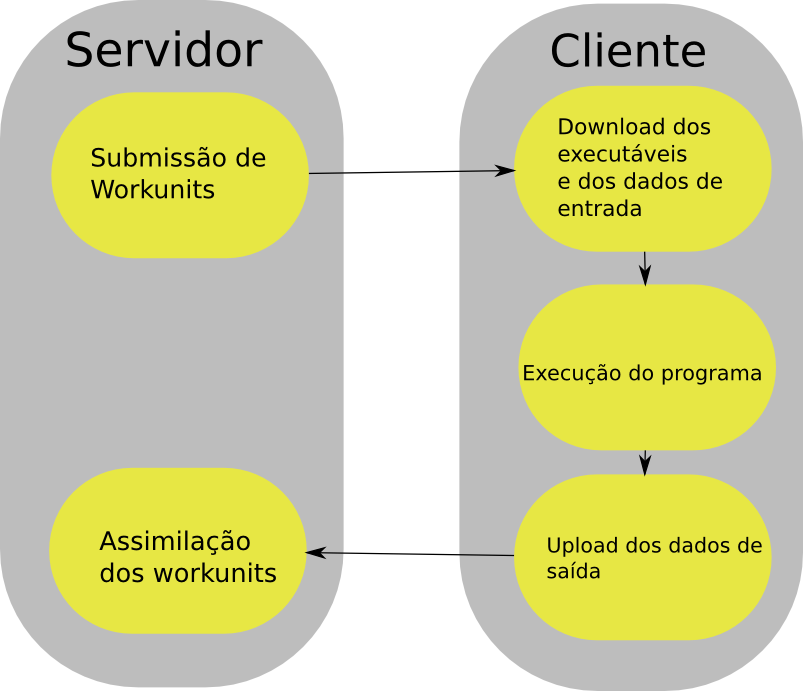
\includegraphics[scale=0.7]{boinc-schema.png}
  \caption{Funcionamento do \textit{BOINC}}
  \label{boinc_funcionamento}
\end{figure}


\section{Funcionamento do BOINC com a linguagem \textit{R}}



O \textit{BOINC} funciona da seguinte maneira: criado um \textit{workunit} que é um conjunto de dados de entrada para uma aplicação, 
o cliente se conecta no servidor, faz o download dos arquivos executáveis da aplicação e dos dados de entrada. Após isso, 
os arquivos são executados com a entrada. Quando o processamento acaba, o cliente faz o upload da saída
e o servidor faz a assimilação da saída, colocando as informações em um banco de dados. O funcionamento do Boinc pode ser visto 
na figura \ref{boinc_funcionamento}. O \textit{wrapper} funciona na etapa de processamento: seguindo
uma configuração em um arquivo XML, o \textit{wrapper} executa um programa que executa o interpretador R junto com
o script em \textit{R}.


\begin{figure}[!h]
  \centering
  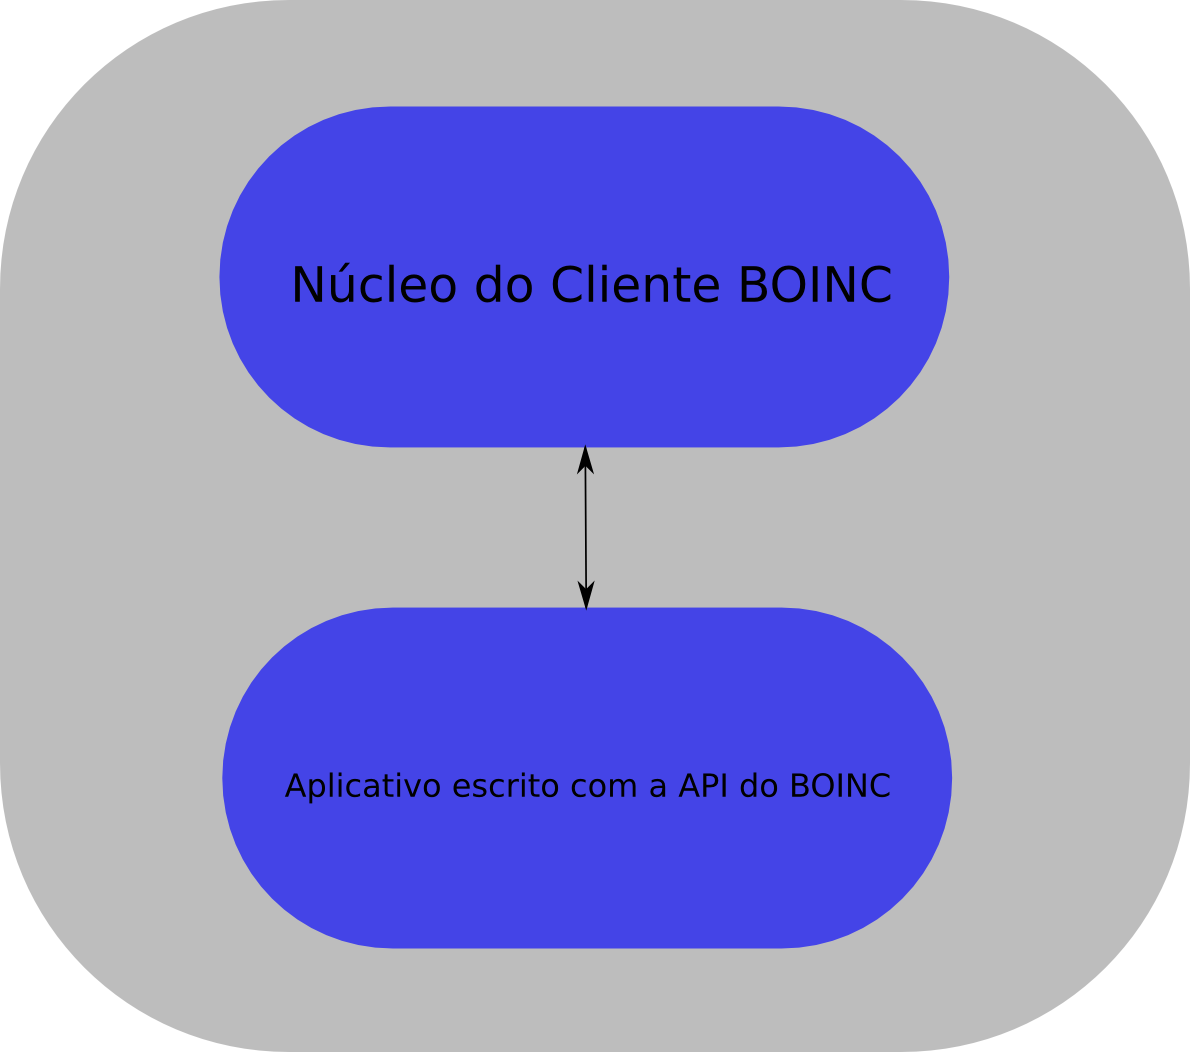
\includegraphics[scale=0.4]{boinc-diagram-normal.png}
  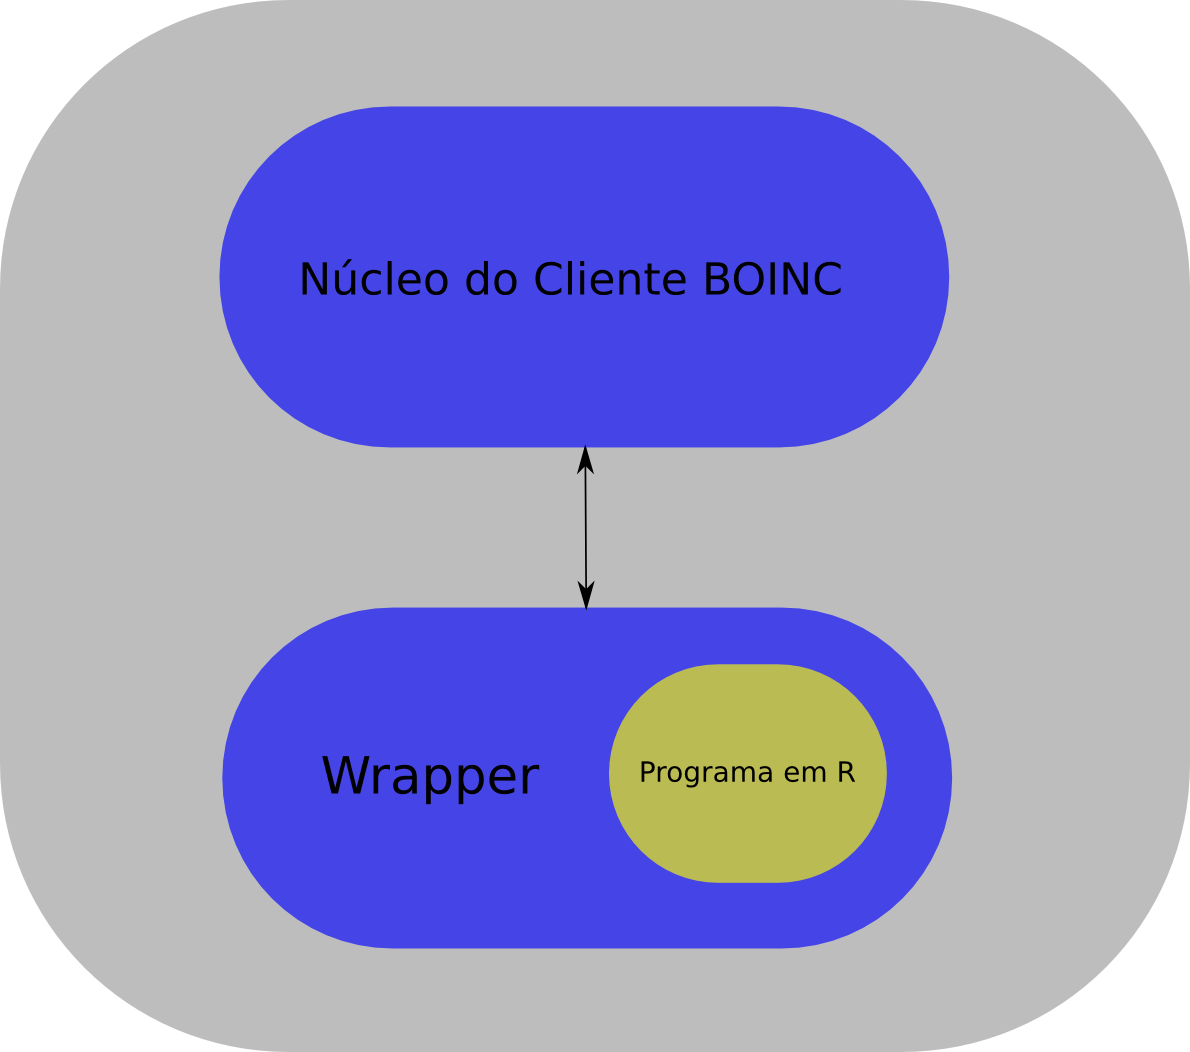
\includegraphics[scale=0.4]{boinc-diagram-wrapper.png}
  \caption{Funcionamento do \textit{BOINC} com um aplicativo usando a API e com o \textit{Wrapper}}
  \label{boinc_funcionamento_nw}
\end{figure}


\section{Resultados e discussão}

A parte do servidor já está implementada e em funcionamento. A instalação
dos clientes está em fase de implantação na Rede CEC do IME-USP e em breve 
a grade estará em seu pleno funcionamento.

A instalação do servidor foi simples: havia um bom guia de instalação e configuração
para o \textit{Debian GNU/Linux}. Porém, a maior dificuldade foi conseguir executar os programas em 
\textit{R} já que haviam bugs na configuração de compilação do \textit{wrapper} para o Windows, e o 
\textit{BOINC} não possuía mensagens de erro que nos permitiam facilmente encontrar o problema. 

\section{Conclusão}
 
O objetivo está bem próximo de ser concluído: só é necessário terminar a implantação
na rede e fazer o anúncio pedindo trabalhos para serem executados na grade. Outro ponto
interessante é que é possível ajudar no processamento usando tanto máquinas com sistemas
Linux quanto Windows o que não foi feito nos outros trabalhos semelhantes citados no projeto.  

Esperamos que a grade seja de grande ajuda a grupos de bioinformática que precisem de recursos
computacionais para fazer análises de dados. 
 
%%% References

%% Note: use of BibTeX als works!!

\bibliographystyle{amsalpha}
\bibliography{bibliografia}


\end{multicols}

\end{document}

